\section{Dynkin Diagrams}

\begin{frame}{Simple Roots \& Dynkin Diagrams}
    To generalize beyond $rank=2$, we must identify the "basis" vectors.
    We define \textbf{Simple Roots} ($\Delta \subset \mathcal{R}$) as positive roots that cannot be decomposed into a sum of other positive roots.

    \vspace{0.3cm}
    \textbf{Definition 4.4.5 (Dynkin Diagrams):} A graph encoding the geometry of $\Delta$:
    \begin{itemize}
        \item \textbf{Nodes:} Each simple root is a node.
        \item \textbf{Edges:} Nodes are connected by $\ell_{\alpha\beta} = 4 \cos^2 \theta_{\alpha\beta} \in \{0,1,2,3\}$ lines.
        \item \textbf{Arrows:} If lengths differ ($\ell > 1$), an arrow points from the longer root to the shorter one ($>$).
    \end{itemize}

    \vfill
    \hyperlink{backup_simpleroots}{\beamerbutton{Formal Def 4.4.3: Simple Roots}}
\end{frame}

\begin{frame}{Dynkin Diagrams for Rank-2}
    \begin{figure}
        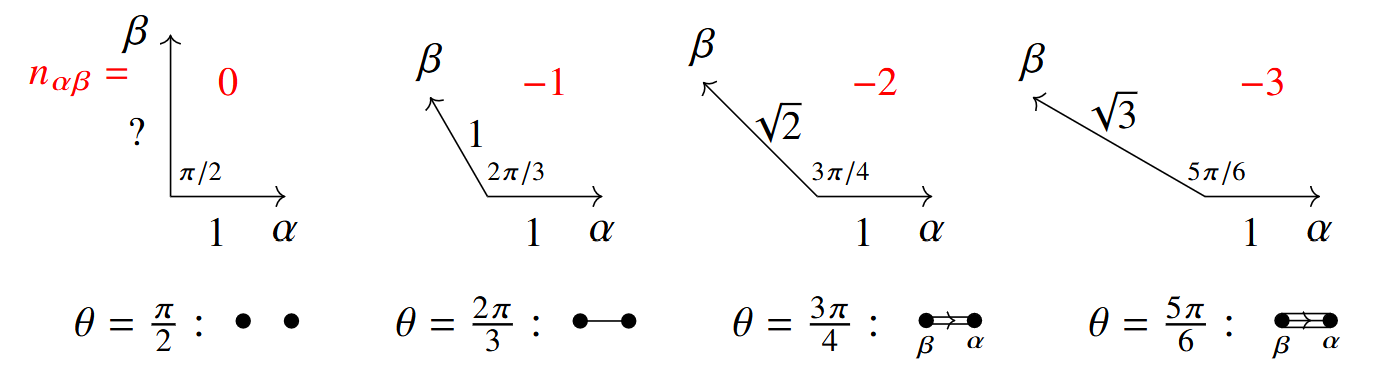
\includegraphics[width=0.8\textwidth]{img/dynkin-blocks.png}
    \end{figure}

    % VOCAL CUE: Spiega che questi 4 mattoncini sono gli unici legami permessi tra NODI ADIACENTI in qualsiasi algebra di Lie di qualsiasi dimensione.
    These 4 fundamental building blocks encode the entire Cartan matrix $C_{ij} = n_{\alpha^{(j)}\alpha^{(i)}}$.
\end{frame}